% Compile from this directory with: make
% XeLaTeX; English and Chinese text are both supported.
\documentclass[10pt,twocolumn,letterpaper]{article}

\usepackage[margin=0.75in,columnsep=0.25in]{geometry}
\usepackage{fontspec}
% Load by filename so macOS does not need these fonts registered in Font Book.
\setmainfont{texgyretermes-regular.otf}[
  BoldFont=texgyretermes-bold.otf,
  ItalicFont=texgyretermes-italic.otf,
  BoldItalicFont=texgyretermes-bolditalic.otf]
\setsansfont{texgyreheros-regular.otf}[
  BoldFont=texgyreheros-bold.otf,
  ItalicFont=texgyreheros-italic.otf,
  BoldItalicFont=texgyreheros-bolditalic.otf]
\setmonofont{lmmono10-regular.otf}
\usepackage[UTF8,scheme=plain,fontset=fandol]{ctex}
\usepackage{amsmath,amssymb}
\usepackage{graphicx}
\usepackage{booktabs}
\usepackage{tabularx}
\usepackage{microtype}
\usepackage{flushend}
\usepackage{titlesec}
\usepackage{xurl}
\usepackage{tikz}
\usepackage[hidelinks]{hyperref}

\raggedbottom
\titleformat{\section}{\large\bfseries}{\thesection}{0.6em}{}
\titleformat{\subsection}{\normalsize\bfseries}{\thesubsection}{0.6em}{}
\titlespacing*{\section}{0pt}{2ex plus .5ex minus .2ex}{.8ex plus .2ex}
\titlespacing*{\subsection}{0pt}{1.5ex plus .3ex minus .2ex}{.5ex plus .2ex}

\title{When Does Cross-Adapter KV Cache Sharing Pay Off?\\
  \large A Study of Multi-Role Coding Agents}
\author{RoleKV}
\date{\today}

\begin{document}
% The title and abstract span both columns; the body starts in two columns.
\twocolumn[\begin{@twocolumnfalse}
\maketitle

\begin{abstract}
This report studies when sharing key-value (KV) caches across role-specific
adapters reduces the cost of multi-role coding agents. We examine the trade-offs
among task quality, end-to-end latency, and memory under different context
lengths, output lengths, and role-switching patterns.
% Add measured findings only after the experiments have been completed.
\end{abstract}
\vspace{1em}
\end{@twocolumnfalse}]

\section{Introduction}
An iterative coding session accumulates more than a problem statement: each
attempt adds code, test output, and feedback that later invocations must
consider. Execution-guided refinement can improve generated programs
\cite{chen2023selfdebug}, motivating a workflow in which a Coder proposes a
solution and a Reviewer decides whether it needs revision. One way to
specialize these roles is to train a LoRA adapter for each on a shared
backbone \cite{hu2022lora}. Although this shares most model weights, the
adapters can produce incompatible key-value (KV) states for the same text
\cite{greenewald2025alora}. A role switch can consequently require processing
shared history under the incoming adapter or maintaining a private cache for
each role.

Cross-adapter cache sharing offers several ways to reduce this duplication.
Activated LoRA (aLoRA) leaves pre-invocation states unchanged, while ICaRus
uses a shared logical encoder to maintain reusable states during generation
\cite{greenewald2025alora,woo2026icarus}. Approximate approaches such as
LRAgent instead share cache components across adapted models
\cite{jeon2026lragent}. These methods establish mechanisms for reuse, but
evaluating them in a coding loop also requires accounting for the work of
maintaining a reusable representation and the quality of the resulting
programs.

The balance depends on the workload and the comparison baseline. A long
shared context creates repeated prefill work, whereas long role outputs add
decoding cost and may require substantial recomputation at handoff. Private
warm caches can avoid rebuilding a returning role's entire history when
memory permits; a single multi-role adapter avoids cross-adapter
incompatibility. Moreover, a method that approves incorrect code early can
appear cheap simply because it stops sooner. These considerations motivate
our central question: \emph{under task-quality and memory constraints, when
does cross-adapter KV cache sharing reduce the actual cost of completing a
coding task?}

We plan a controlled study of a small-model Coder--Reviewer loop on MBPP
function-level tasks \cite{austin2021mbpp}, augmented with shared code context.
The study will compare aLoRA handoffs that rebuild base-model states (H1) or
retain adapted states (H2), alongside full recomputation, private warm caches,
and a single multi-role adapter. Numerical checks against full recomputation
with the same aLoRA weights will verify H1's cache correctness. Fixed-trace
measurements will isolate processing costs as context length, output length,
and switch frequency vary; closed-loop runs will assess final correctness,
repair, regression, and Reviewer decisions. The intended contribution is an
empirical characterization of when saved prefill work translates into lower
task cost at acceptable quality, with canonicalization, decoding, and tool
execution included in the accounting.

\section{Background and Related Work}
\label{sec:background}

\subsection{Code Repair and Shared History}
Iterative code repair revisits a task together with earlier programs and their
execution results. Self-Debugging uses generation, explanation, feedback, and
revision to improve code with an existing language model
\cite{chen2023selfdebug}. Its MBPP evaluation exposes one test and reserves
two for final scoring: execution feedback can reveal a failure, while passing
the visible test leaves further errors undetected. This motivates a
Coder--Reviewer loop in which both roles inspect a growing common history.
The benefit of separate role adapters remains an empirical question, since a
single model can also perform generation and review.

\subsection{LoRA and KV Compatibility}
LoRA specializes a frozen backbone through trainable low-rank weight updates
\cite{hu2022lora}. S-LoRA makes many such adapters practical to serve through
heterogeneous batching and unified memory management for adapter weights and
KV tensors \cite{sheng2024slora}. These optimizations exploit shared backbone
weights; cross-adapter KV reuse additionally requires compatible activations.
An adapter can change cached keys and values directly through projection
updates or indirectly through hidden states produced by earlier layers
\cite{greenewald2025alora}.

Ordinary autoregressive caching retains earlier keys and values during
decoding. vLLM's PagedAttention manages these tensors in blocks and supports
sharing within and across requests \cite{kwon2023pagedattention}. With an
unchanged model and compatible positions, identical prefixes can reuse their
states. Identical text under different adapters does not generally satisfy
that condition. The resulting trade-off depends on cache policy: full
recomputation uses one live cache, whereas private warm caches retain a prefix
for each role and compute its missing history on return. Cross-adapter sharing
must therefore be assessed against both recomputation cost and the memory
required to keep private caches resident.

\subsection{Exact Cross-Adapter Sharing}
Activated LoRA (aLoRA) preserves base-model states before an invocation
sequence and applies adaptation from that sequence onward
\cite{greenewald2025alora}. This enables exact reuse of the base-processed
prefix. Li et al. integrate the mechanism into vLLM through base-aligned block
hashing and activation-aware masking \cite{li2025aloraserving}. The boundary
is important for sequential role invocations: the aLoRA paper notes that
adapter-generated states cannot be directly reused by another adapter or the
base model, so the generated text must be prefilled again. Our H1 policy
applies this recomputation at handoff, including the adapted role header.

ICaRus takes a different approach: it freezes a shared logical encoder that
writes KV states and trains task-specific logical decoders that read them
\cite{woo2026icarus}. During generation, the base and adapted paths run
together, with shared weight reads and combined attention queries reducing
their execution overhead. Thus, ICaRus maintains reusable states throughout
decoding, whereas H1 reconstructs them in a contiguous pass at handoff.
ICaRus evaluates code-generation quality and HotpotQA-based serving workloads;
those experiments do not directly measure our code-repair loop. In both
architectures, exact cache reuse concerns states under the chosen adaptation
design; task quality relative to conventional LoRA requires separate evaluation.

\subsection{Approximate Sharing and Reconstruction}
Other approaches reuse representations across model variants while managing
the resulting mismatch. DroidSpeak selectively recomputes layers of another
variant's cache and reuses the rest \cite{liu2026droidspeak}. LRAgent instead
decomposes the value cache into a shared base component and a compact
adapter-dependent component \cite{jeon2026lragent}. BaseShared maintains
per-agent low-rank caches for standard adapters; BaseLRShared further shares
the low-rank cache using a shared-$A$ adapter architecture. Sharing the base
weights alone does not make the base component identical, because its input
hidden states can still depend on the producing adapter.

ForkKV combines disaggregated shared and agent-specific caches with a
DualRadixTree and a reconstruction kernel for multi-LoRA serving
\cite{wang2026forkkv}. PReCache precomputes each adapter's low-rank cache;
its ReBaseShared variant additionally constructs a neutral base cache from
adapter-free hidden states \cite{jeon2026precache}. The lazy-prefill schedule
performs this reconstruction after an agent's turn. This resembles H1 in
scheduling base-state reconstruction at a handoff, but serves a different
purpose: PReCache approximates standard adapters' representations, whereas
H1 restores the base prefix expected by the incoming aLoRA. These distinctions
separate the choice of reusable representation from the cost of maintaining it.

\subsection{Scope and Measurement}
Prior work establishes both exact and approximate paths to cross-adapter
sharing. We examine its benefit in a small-model Coder--Reviewer workload,
focusing on aLoRA handoffs. H1 rebuilds the previous role's
adapted states with base weights; H2 retains them, trading that work for a
mismatch with our base-prefix training setup. The question is how shared
context length, role-output length, and switching frequency affect the
quality--cost trade-off, including canonicalization and decoding overhead.

We plan to compare H1 and H2 with full recomputation, private warm caches,
and a single multi-role adapter. Controlled traces isolate cache-processing costs,
while closed-loop runs capture how code, review decisions, and session length
change together. PReCache likewise distinguishes controlled efficiency traces
from actual agent trajectories \cite{jeon2026precache}. We use both forms of
measurement to test when savings in repeated prefill translate into lower task
cost at acceptable quality. The other sharing systems reviewed here provide
context for this study. Section~\ref{sec:methods} describes the planned protocol.

\section{Research Questions}
\begin{enumerate}
  \item How do shared context length, role output length, and switch frequency
    affect the benefit of sharing?
  \item How do cache handoff policies affect task quality and total task cost?
  \item When is sharing preferable to retaining a private cache for each role
    or using a single multi-role adapter?
\end{enumerate}

\section{Methods and Experimental Design}
\label{sec:methods}
We distinguish the data and runtime present in the inspected repository from
the training recipe and comparisons still awaiting run-level confirmation.
Results will identify the checkpoints, feedback protocol, and policies actually
evaluated. The source and data hashes used for this description are recorded
in \path{report/methods_manifest.json}.

\subsection{Tasks and Shared Context}
The target model is Qwen2.5-Coder-1.5B-Instruct
\cite{hui2024qwen25coder}; the 0.5B variant is used for development. The task
loader uses MBPP's \texttt{full} configuration \cite{austin2021mbpp}, pooling
the train, validation, and prompt splits for data generation and selecting
100 test-split tasks with Python's random sampler at seed 0. It checks that
the training and selected evaluation task IDs are disjoint.

Each TASK segment contains a repository-style \texttt{utils.py}, the task
description, and its first assert. The context builder samples 30 reference
solutions from the pooled training tasks by default, excluding the target
task; selection is deterministic from a hash of the task ID. These functions
provide shared text to process, not evidence that the task requires a real
repository. In the current SFT exports, TASK segments range from 1,276 to
2,497 development-tokenizer tokens, with a median of approximately 1,809.
The added context and evaluation subset are study-specific augmentations.

\subsection{Teacher Trajectories and SFT Examples}
The generator requests a solution or an intentionally faulty first attempt
from a teacher, executes the code, and retains a trajectory only if its final
code passes the full assert suite. A requested faulty attempt must fail that
suite; its feedback is generated from the real test output, followed by a
tested repair. Passing attempts receive a deterministic \texttt{APPROVE}
target. The configured teacher identifier is \texttt{claude-sonnet-5-5}; the
export does not record the API model revision or generation arguments, so
these remain provenance information to recover from the generation run.

The current export contains 280 accepted trajectories from distinct tasks:
222 Coder--Reviewer sequences and 58 Coder--Reviewer--Coder repair sequences.
They yield 338 Coder and 280 Reviewer SFT rows, with 222 \texttt{APPROVE} and
58 \texttt{REVISE} labels. The Coder file retains the 58 faulty initial
attempts as targets as well as their repairs; it represents trajectory
imitation, not exclusively correct-solution supervision. No Reviewer turn
after a successful repair is included in these three-turn trajectories.
The accepted distribution therefore differs from the generator's nominal
50\% bug-request default.

Prompts use separately tokenized ChatML segments. The system segment is shared
with inference, and a role's complete assistant header is its aLoRA invocation
sequence. Labels mask all context tokens with $-100$ and supervise only the
target BODY, including its closing delimiter. The two files' median lengths
are 2,036 and 2,060.5 tokens for Coder and Reviewer, respectively; the maximum
is 2,932. These lengths were checked locally using the development tokenizer.
Full data hashes appear in the manifest and \texttt{data/README.md}.

\subsection{Adapter Training Recipe}
The team recipe specifies role-specific standard LoRA and aLoRA adapters,
plus a shared LoRA trained on both roles for A1. Table~\ref{tab:training-recipe}
records the prescribed settings. Only the seven attention and MLP linear
projections are targeted; embeddings and the language-model head are excluded
to preserve the base-prefix sharing assumptions. Loss is computed only on
the role's target tokens.

\begin{table}[htbp]
\centering
\small
\begin{tabularx}{\columnwidth}{@{}>{\raggedright\arraybackslash}p{0.43\columnwidth}>{\raggedright\arraybackslash}X@{}}
\toprule
Setting & Prescribed value \\
\midrule
Standard LoRA / aLoRA rank & 16 / 32 \\
Scaling $\alpha$ & $2r$ \\
Targets & q, k, v, o, gate, up, down projections \\
Learning rate / epochs & $2\times 10^{-4}$ / 2 \\
Maximum sequence length & 4,096 tokens \\
Precision / checkpointing & bf16 / gradient checkpointing \\
Reviewer REVISE multiplicity & $3\times$ (team run setting) \\
\bottomrule
\end{tabularx}
\caption{Training recipe from the team documents, pending verification against
actual training arguments and checkpoint configurations.}
\label{tab:training-recipe}
\end{table}

REVISE oversampling repeats those Reviewer examples in the training input,
including when training the shared adapter; it leaves the exported data files
unchanged. The inspected checkout does not contain the training script,
checkpoint configurations, or training logs. Optimizer, batching, scheduling,
seeds, completed epochs, and actual hyperparameters must therefore be reported
from the training runs before quality results are attributed to this recipe.
The unequal prescribed ranks also preclude describing the comparison as
parameter-matched.

\subsection{Session Protocol and Test Feedback}
The runtime follows Coder $\rightarrow$ tool output $\rightarrow$ Reviewer.
It uses greedy decoding with default limits of 512 new Coder tokens and
128 Reviewer tokens, stopping on ChatML end-of-turn or end-of-text tokens.
An \texttt{APPROVE} or \texttt{INVALID} Reviewer verdict ends the session.
After the second \texttt{REVISE}, the next Coder output is final, without a
further tool call or review, for at most five role turns. Tests execute in a
temporary-directory Python subprocess with a five-second timeout and an
output cap of 2,000 characters.

\paragraph{Feedback boundary.}
Although only the first assert appears in the TASK text, the current data
generator and default evaluation runner execute \emph{all} MBPP asserts in
the tool call and return the resulting stdout and stderr to the model.
Final code is scored against the same suite. These are test-suite-assisted
repair results, not evaluation on tests withheld throughout the interaction;
failure output can reveal additional assertions. A runner option restricts
feedback to the first assert, matching the visibility boundary used by
Self-Debugging \cite{chen2023selfdebug}, but that is a separate protocol whose
runs must be labeled and analyzed separately. Comparisons must hold the
feedback policy fixed, and equal feedback access does not establish
generalization to unseen tests.

\subsection{Cache Policies and Correctness}
The implemented runtime uses one logical token history and one
\texttt{DynamicCache} per session, with the following policies:
\begin{itemize}
  \item \textbf{A2 (full recomputation):} discard the cache at each turn and
    prefill the entire history and new role header under the incoming role's
    standard LoRA.
  \item \textbf{A5-H1 (canonicalize):} retain the base-processed prefix, crop
    the previous role's adapted span, and rebuild it with base weights at
    the start of the next turn. This covers the previous role's header and
    output. New tool and boundary tokens are processed in the same forward;
    the incoming aLoRA activates only at its own header. The final session
    turn is never canonicalized because there is no subsequent handoff.
  \item \textbf{A5-H2 (keep):} retain the previous role's adapted KV, process
    new input, and activate the incoming aLoRA at its header. The resulting
    history contains states produced by different adapters.
\end{itemize}
All aLoRA decode steps receive explicit activation offsets so that adaptation
remains active when the input chunk no longer contains the invocation header.
A0 uses the base model, A1 uses one shared standard LoRA, and A3 retains
mixed-adapter history with standard role LoRAs; these policies also have
runtime implementations. H1 and H2 will use the same aLoRA weights.

Inference uses PEFT 0.21.2 with scaled dot-product attention. A contiguous-slice
aLoRA path and persistent activation-offset hooks replace masked row selection
and per-call hook registration. Timings characterize this optimized runtime;
numerical checks must cover activation behavior and cache policy at the
measured precision.

\begin{figure*}[tbp]
\centering
% Editable vector schematic. Spans have equal widths for layout, not token counts.
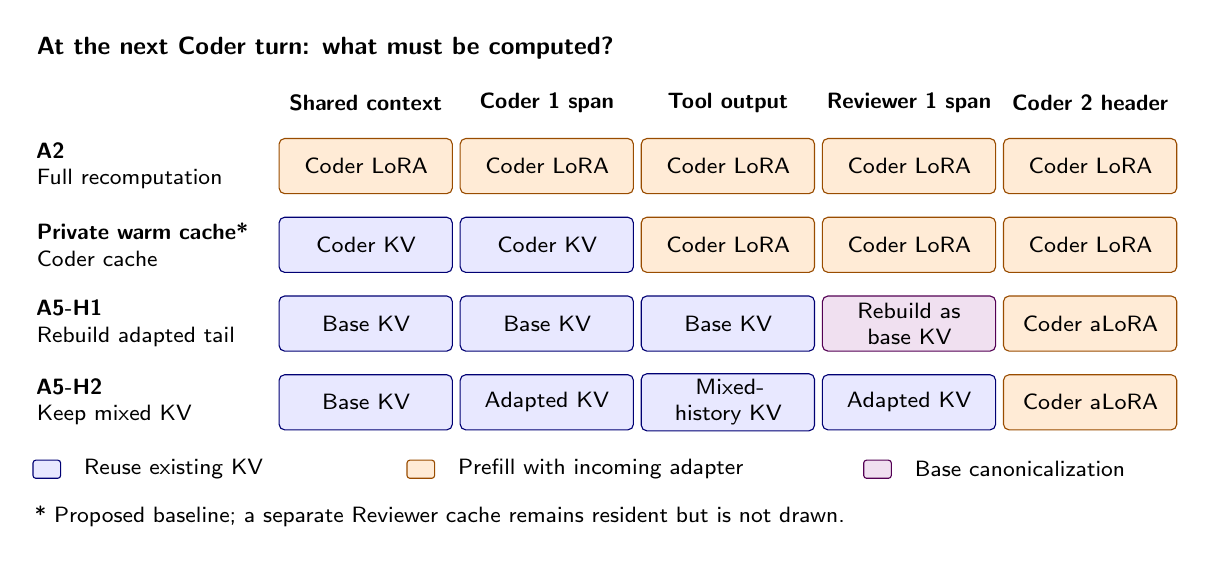
\begin{tikzpicture}[
  x=1cm,y=1cm,font=\sffamily\footnotesize,
  box/.style={draw,rounded corners=2pt,minimum width=2.2cm,
    minimum height=.70cm,text width=2.04cm,align=center,inner sep=2pt},
  swatch/.style={draw,rounded corners=1pt,minimum width=.35cm,
    minimum height=.23cm,inner sep=0pt},
  reuse/.style={box,draw=blue!45!black,fill=blue!9},
  work/.style={box,draw=orange!60!black,fill=orange!16},
  canon/.style={box,draw=violet!65!black,fill=violet!12}
]
\node[anchor=west,font=\sffamily\small\bfseries] at (0,.95)
  {At the next Coder turn: what must be computed?};
\foreach \x/\name in {4.3/Shared context,6.6/Coder 1 span,
  8.9/Tool output,11.2/Reviewer 1 span,13.5/Coder 2 header}
  \node[align=center,font=\sffamily\footnotesize\bfseries] at (\x,.25) {\name};

\node[anchor=west,align=left,text width=2.8cm] at (0,-.55)
  {\textbf{A2}\\Full recomputation};
\foreach \x in {4.3,6.6,8.9,11.2,13.5}
  \node[work] at (\x,-.55) {Coder LoRA};

\node[anchor=west,align=left,text width=2.8cm] at (0,-1.55)
  {\textbf{Private warm cache*}\\Coder cache};
\foreach \x in {4.3,6.6}
  \node[reuse] at (\x,-1.55) {Coder KV};
\foreach \x in {8.9,11.2,13.5}
  \node[work] at (\x,-1.55) {Coder LoRA};

\node[anchor=west,align=left,text width=2.8cm] at (0,-2.55)
  {\textbf{A5-H1}\\Rebuild adapted tail};
\foreach \x in {4.3,6.6,8.9}
  \node[reuse] at (\x,-2.55) {Base KV};
\node[canon] at (11.2,-2.55) {Rebuild as\\base KV};
\node[work] at (13.5,-2.55) {Coder aLoRA};

\node[anchor=west,align=left,text width=2.8cm] at (0,-3.55)
  {\textbf{A5-H2}\\Keep mixed KV};
\node[reuse] at (4.3,-3.55) {Base KV};
\node[reuse] at (6.6,-3.55) {Adapted KV};
\node[reuse] at (8.9,-3.55) {Mixed-history KV};
\node[reuse] at (11.2,-3.55) {Adapted KV};
\node[work] at (13.5,-3.55) {Coder aLoRA};

\node[swatch,draw=blue!45!black,fill=blue!9] at (.25,-4.4) {};
\node[anchor=west] at (.6,-4.4) {Reuse existing KV};
\node[swatch,draw=orange!60!black,fill=orange!16] at (5.0,-4.4) {};
\node[anchor=west] at (5.35,-4.4) {Prefill with incoming adapter};
\node[swatch,draw=violet!65!black,fill=violet!12] at (10.8,-4.4) {};
\node[anchor=west] at (11.15,-4.4) {Base canonicalization};
\node[anchor=west,align=left,text width=14.6cm,font=\sffamily\footnotesize]
  at (0,-5.0) {* Proposed baseline; a separate Reviewer cache remains resident but is not drawn.};
\end{tikzpicture}

\caption{Cache preparation on returning to the Coder. Equal-width columns
denote logical spans, not measured cost; boundary tokens are omitted. H1
rebuilds Reviewer~1's adapted span after Coder~1 was canonicalized at the
preceding handoff. H2 keeps mixed-adapter KV. Private warm caches (proposed)
also retain a separate Reviewer cache.}
\label{fig:cache-handoff}
\end{figure*}

Private warm caches remain unimplemented in the inspected runtime. The
proposed policy keeps a valid prefix per standard role adapter and computes
missing history on return. Its comparison with A2 must use identical adapters
and count all resident caches. Figure~\ref{fig:cache-handoff} illustrates
policies independently of checkpoint quality.

A full-recomputation run of the \emph{same aLoRA} will serve as H1's numerical
correctness reference, using identical input histories. Cache states and
logits will be checked at handoffs and decode steps with precision-appropriate
tolerances before timing is trusted. Ordinary LoRA is a separate task-quality
reference, not an equivalence target. H2 intentionally changes cache semantics
and will be assessed for quality rather than required to pass H1 equivalence.

\subsection{Fixed-Trace System Measurements}
We will replay identical role outputs and tool segments for every cache policy
to isolate processing costs. Controlled sweeps will vary shared-context length,
output length, and the number of role switches within the session protocol.
These prescribed traces cannot establish task quality. Measurements will count
all computed prefill tokens, including H1 canonicalization, and report
post-switch time to first token and decoding time per token. Repeated runs will
alternate policy order on the same GPU after warm-up and report timing spread.

Memory results will distinguish logical cache size at turn boundaries from
the measured runtime peak. Private-cache comparisons will count every live
cache under the same GPU memory budget. Memory savings will not be inferred
from prefill-token savings or claimed against A2 solely because H1 shares a
prefix.

\subsection{Quality and Reviewer Behavior}
In a separate evaluation, each method will generate its own code and reviews
on the same task set. We will report initial-Coder and final-code pass rates,
turn counts, actual role-switch counts, and invalid or truncated outputs.
For diagnostic scoring, intermediate code may additionally be evaluated after
the run against the full test suite, without exposing these additional
post-hoc outcomes to either role. This does not make the suite held out when
the all-assert feedback protocol is used.
The following quantities will be reported with their numerator and denominator:
\begin{itemize}
  \item \textbf{Task repair rate:} initially failing tasks whose final code
    passes, divided by all initially failing tasks.
  \item \textbf{Task regression rate:} initially passing tasks whose final code
    fails, divided by all initially passing tasks.
  \item \textbf{False-approval rate:} approvals of code that passes the first
    assert but fails the full suite, divided by approvals of code passing that
    first assert. Under all-assert feedback, this measures review behavior
    with suite-derived feedback, not hidden-test generalization.
\end{itemize}
Undefined rates will be marked as such when their denominator is zero.
Turn-level repair and regression analysis will additionally examine code pairs
separated by a revision request, reporting how many cases reached that stage.
We will keep stopped, invalid, and failed sessions in the task-level results
rather than compare only sessions that complete the longest loop.

\subsection{Cost--Quality Interpretation}
Closed-loop methods may take different trajectories, so fewer processed tokens
can reflect premature approval or failure rather than a better cache policy.
We will interpret cost jointly with task success and Reviewer behavior, using
paired task comparisons. Model-turn time (the sum of logged turn durations)
will be distinguished from end-to-end task wall time, which also includes tool
execution and orchestration. Lower prefill counts alone will not be reported
as an end-to-end speedup. Uncertainty and sample counts will accompany quality
differences; a small observed gap will not establish equivalence.

\section{Results and Analysis}
% Add measured results with hardware, configuration, seeds, and uncertainty.
% Plot the regimes in which each strategy is preferable.
% Do not interpret fewer prefill tokens as an automatic end-to-end speedup.

\section{Limitations and Discussion}
% Discuss synthetic context, task/model coverage, and generalization.
% Do not infer unpublished implementation details of commercial coding agents.

\section{Conclusion}
% Summarize supported findings and practical guidance after evaluation.

\bibliographystyle{unsrt}
\begingroup
\raggedright
\bibliography{references}
\endgroup

\end{document}
